\documentclass{homework}

\title{Modern Final}
\author{Kevin Evans}
\studentid{11571810}
\date{May 7, 2020}
\setclass{Physics}{304}
\usepackage{amssymb}
\usepackage{mathtools}

\usepackage{amsthm}
\usepackage{amsmath}
\usepackage{slashed}
\usepackage{relsize}
\usepackage{threeparttable}
\usepackage{float}
\usepackage{booktabs}
\usepackage{boldline}
\usepackage{changepage}
\usepackage{physics}
\usepackage[inter-unit-product =\cdot]{siunitx}
\usepackage{setspace}

\usepackage[makeroom]{cancel}
\usepackage{pgfplots}

\usepackage{multicol}
\usepackage{tcolorbox}
\usepackage{enumitem}
\usepackage{times}
\usepackage{mhchem}
\usepackage{graphicx} 
\DeclareSIUnit{\year}{yr}
\usepackage[export]{adjustbox}

\usepackage{dsfont}
\newcommand{\1}{\mathds{1}}

\begin{document}
	\maketitle
	\begin{enumerate}[label={\arabic*.}]
		\item For spin-$\frac{1}{2}$ particles, e.g. electrons, each energy state would be limited to two particles per state\footnote{Due to the Pauli exclusion principle arising from the indistinguishably of particles.}. Then, for a one-dimensional box of length $L$, the energy of each state is \begin{align*}
			E_n & = \frac{p_n^2}{2m} = \frac{\hbar^2 \pi^2 n^2}{2 m L}
		\end{align*}
		So, for five particles, they would occupy the first three states: $2$ in $E_1$, $2$ in $E_2$, and $3$ in $E_3$. The total energy is then \begin{align*}
			E_\mathrm{tot} & = E_1 + E_2 + E_3 \\
				& = \frac{\hbar^2 \pi}{2 mL} \left(2 \times 1^2 + 2 \times 2^2 + 1 \times 3^2\right) \\
				& = 19 \frac{\hbar^2 \pi^2}{2 mL}
		\end{align*}
	
		\item For spin-$1$ particles, like photons, they would all occupy the ground state $n=1$, \begin{align*}
			E_\mathrm{tot} & = 5 \times E_1 \\
				& = 5 \frac{\hbar^2 \pi^2}{2 mL}
		\end{align*}
	
		\item A similar result would be observed with a neutron since it is spin-$\frac{1}{2}$. In the original experiment, electronically-neutral silver atoms were used. The result of the Stern-Gerlach experiment was due to the intrinsic spin moment and the torque experienced by the particles, $\bvec{\mu}_\mathrm{s} \cross \bvec{B}$.
		
		\item For the $3d$ electron, $n=3$, $\ell=2$, $s = \frac{1}{2}$, \begin{align*}
			j & = \left\{ \frac{5}{2}, \frac{3}{2} \right\} \\
			m_j & = \left\{ \pm \frac{5}{2}, \pm \frac{3}{2}, \pm \frac{1}{2} \right\} & \text{For } j = \frac{5}{2} \\
				& = \left\{ \pm \frac{3}{2}, \pm \frac{1}{2}\right\} & j = \frac{3}{2}
		\end{align*}
		
		\clearpage
		
		\item \begin{enumerate}
			\item \underline{Theorem}
					
				$$\sum_{n=0}^{\infty} x^n = \frac{1}{1 - x}$$
			
				\underline{Proof}
				\begin{align*}
					S(x) & = \sum_{n=0}^{\infty} x^n \\
					x S(x) & = x \left( \sum_{n=0}^\infty x^n \right) = \sum_{n=0}^\infty x^{n+1} = \sum_{n=1}^\infty x^n = S(x) - 1 \\
						x S(x) - S(x) & = -1 \\
						\left( x - 1 \right) S(x) & = -1 \\
						S(x) & = \frac{1}{1 - x} && \qed
				\end{align*}
			
			\item \underline{Theorem}
				
				$$\sum_{n=0}^\infty nx^n = \frac{x}{\left(1 - x\right)^2}$$
				
				\underline{Proof}
				\begin{align*}
					S(x) & = \sum_{n=0}^\infty x^n = \frac{1}{1-x} && \text{From (a)} \\
					\dv{x} S(x) & = \sum_{n=0}^{\infty} n x^{n-1} = \frac{1}{(1-x)^2} \\
					x \left( \dv{x} S(x) \right) & = \sum_{n=0}^{\infty} n x^{n} = \frac{x}{(1-x)^2} && \qed
				\end{align*}
		\end{enumerate}
	
		\clearpage
		
		\item For a harmonic oscillator, the energy of the $n$-th state is
			\[ E_n = \left( n + \frac{1}{2} \right) \hbar \omega \]
			If we consider the denominator and numerator sums separately and substitute this energy in, \begin{align*}
				D & = \sum_{n}^{\infty} e^{-E_n / k_B T}
					= \sum_{n}^\infty e^{ -\left(n + 1/2 \right) \hbar \omega / k_B T} \\
				& = e^{ - \hbar \omega / 2 k_B T} \sum_{n}^\infty  \left(e^{ -\hbar \omega / k_B T} \right)^{n} \\
				& = \frac{e^{ - \hbar \omega / 2 k_B T}}{ 1 - e^{ - \hbar \omega / k_B T}  } \\
				N & = \sum_{n}^{\infty} E_n e^{-E_n / k_B T} \\
					& = \sum_{n}^{\infty} \left( n + \frac{1}{2}\right) \hbar \omega e^{- \left(n + \frac{1}{2}\right) \hbar \omega / k_B T} \\
					& = \hbar \omega e^{-\hbar \omega / 2k_B T} \left[
						\sum_{n}^{\infty} n \left(
							e^{-\hbar \omega / k_B T}
						\right)^n
						+ \frac{1}{2} \sum_{n}^\infty \left(
							e^{-\hbar \omega / k_B T}
						\right)^n
					\right] \\
				& = \hbar \omega e^{-\hbar \omega / 2 k_B T} \left[
						\frac{e^{-\hbar \omega / k_B T}}{\left(1 - e^{-\hbar \omega / k_B T} \right)^2}
						+ \frac{1}{2} \left(\frac{1}{1 - e^{-\hbar \omega / k_B T}}\right)
					\right]
				\intertext{Plugging this back into the $\bar{E}$ fraction and letting $u = e^{-\hbar \omega / k_B T}$,}
				\bar{E} & = \hbar \omega u^{1/2} \left(\frac{u}{\left(1 - u\right)^2} + \frac{1}{2(1 - u)} \right) \frac{1 - u}{u^{1/2}} \\
					& = \hbar \omega \left( \frac{u}{1 - u} + \frac{1}{2} \right) \\
					& = \hbar \omega \left(\frac{1}{e^{\hbar \omega / k_B T} - 1} + \frac{1}{2}\right)
			\end{align*}
		\item For photons, it follows the Bose-Einstein distribution with $\mu = 0$, \[ f(E) = \frac{1}{e^{E/k_B T} - 1} \]
		The density (degeneracy?) $g(E) \propto E^2$ \begin{align*}
			\bar{E} & = \int_{0}^{\infty} E g(E) f(E) \dd{E} \\
				& = k \int_{0}^\infty \frac{E^3}{e^{E / k_B T} - 1} \dd{E}
			\intertext{Letting $u = E / k_B T$, then $\dd{E} = k_B T\dd{u}$}
			\bar{E} & = k \left(k_B T \right)^4 \int_{0}^\infty  \frac{u^3}{e^u - 1} \dd{u}
			\intertext{As the integral converges,}
			\bar{E} & \propto T^4 \qed
		\end{align*}
	
		\item By analyzing the molecule's spectra, we can observe the energies of the optical transitions between $\ell$-values as it absorbs (or emits) photons of certain wavelengths. From these values, we can infer the composition and size of the molecule (like Raman spectroscopy?).
		
		\item As $c = \lambda f$, then \begin{align*}
			f & = c / \lambda \\
			\dd{f} & = - c\dd{\lambda} / \lambda^2
			\intertext{Using this in the reexpression and ignoring the negative in that differential,}
			\dd{U_\mathrm{phot}} & = \frac{hc^3 / \lambda^3}{e^{hc / k_B T \lambda} - 1} \frac{8 \pi V}{c^3} \left(\frac{c \dd{\lambda}}{\lambda^2}\right) \\
				& = \frac{8\pi V hc}{\lambda^5} \frac{ \dd{\lambda}}{e^{hc / k_B T \lambda} - 1} 
		\end{align*}
	
		\item Given the density of states $$g(E) = AE^{1/2}$$
		The number of microstates is given as \begin{align*}
			\Omega & = \int_{0}^{\infty} g(E) \dd{E} = A\int_{0}^\infty E^{1/2} \dd{E} 
			\intertext{As the states above the Fermi level are generally unoccupied at low-ish temperatures, the upper limit is reduced to the Fermi energy $E_F$.}
			\Omega & = A\int_{0}^{E_F} E^{1/2} \dd{E} \\
				& = \eval{ \frac{2A}{3} E^{3/2} }_{0}^{E_F} \\
				& = \frac{2A}{3} {E_F}^{3/2} \qed
		\end{align*}
	
		\item It would be a good conductor despite the $3s$ orbital being filled. From the diagram, there is some overlap between the $3s$ and $3p$ bands which allows electrons to flow across the combined $3s$-$3p$ conduction band.
		
		\item When a photon's energy exceeds the energy gap of a material, it can be absorbed. In diamond, the energy gap is fairly high and requires a higher energy photon, whereas silicon has a relatively low energy gap. A visible light photon has enough energy for absorption by silicon, but not diamond. 
		
		\clearpage
		
		\item If we \textit{only} consider the coefficients for absorption $B_{12}$ and emission $A_{21}$ then as there are a fixed number of atoms in the system, we can equate
		\begin{align*}			
			n_2 A_{21} & = n_1 u(f, T) B_{12} \\
			\frac{n_2}{n_1} & = \frac{B_{12}}{A_{21}} u(f, T)
			\intertext{As it's in thermal equilibrium, we can also relate the populations of the two states as}
			\frac{n_2}{n_1} & = \frac{g_2 (E_2)}{g_1 (E_1)} e^{-hf / k_B T}
			\intertext{Then if we equate these two equations and solve for $u(f, T)$,}
			u(f, T) & = \frac{A_{21}}{B_{12}} \frac{g_2 (E_2)}{g_1 (E_1)} e^{-hf / k_B T}
		\end{align*}
		It's quite clear that this does not match the expected form of the Planck blackbody equation, as it's missing the $-1$ bit capturing the nature of bosons. If we include the stimulated emission coefficient $B_{21}$ then reequate the rates,
		\begin{align*}
			n_2 A_{21} + n_2 u(f, T) B_{21} & = n_1 u(f, T) B_{12} \\
			n_2 \left[A_{21} + u(f, T) B_{21} \right] & = n_1 u(f, T) B_{12} \\
			\frac{n_2}{n_1} & = \frac{u(f, T) B_{12}}{A_{21} + u(f, T) B_{21}} = \frac{1}{\frac{A_{21}}{B_{12} u(f, T)} + B_{21} / B_{12}}
			\intertext{Setting this to the Boltzmann ratio and inverting,}
			\frac{A_{21}}{B_{12} u(f, T)} + B_{21} / B_{12} & = \frac{g_1 (E_1)}{g_2 (E_2)} e^{hf / k_B T} \\
			u(f, T) & = \frac{B_{12} / A_{21}}{\frac{g_1 (E_1)}{g_2 (E_2)} e^{hf / k_B T} - B_{21} / B_{12}}
			\intertext{Including the light-dependent emission term correctly predicts the form of the blackbody equation,}
			u(f, T) & = \frac{B_{12} / A_{21}}{\frac{g_1 (E_1)}{g_2 (E_2)} e^{hf / k_B T} - B_{21} / B_{12}} \sim \frac{hf^3}{e^{hf/k_B T} - 1} \frac{8\pi V}{c^3}
		\end{align*}
		
		\item As the most stable atoms are near the maximum of the chart, fission can release energy through the energy difference between the large parent isotope and its daughter isotopes, i.e. the binding energy. 
		
		\item Larger nuclei require additional neutrons to keep the atom stable as the electrostatic/Coulomb forces can cause an instability from the repulsion of the $p-p$ pairs. For smaller nuclei, nuclear forces can hold the protons in-place and additional neutrons are no longer needed. 
		
		\item If the entirety of the star's mass is now neutrons, \begin{align*}
			r & = r_0 \left(\frac{M_\mathrm{star}}{m_\mathrm{n}}\right)^{1/3} \\
			r & = \SI{1.2}{\femto\meter} \times \left(
				\frac{2\times\SI{1.99e30}{\kg}}{\SI{1.67e-27}{\kg/n}} \right)^{1/3} \\
			& \approx \SI{16}{\km}
		\end{align*}
	
		\item From the uncertainty principle: $\hbar \approx \Delta p \Delta x \leftrightarrow \Delta E \Delta t$, if we assume the velocity $c$, \begin{align*}
			\Delta E & \approx \frac{\hbar}{\Delta T} \approx  \frac{\hbar c}{R} \\
			R & \approx \frac{\hbar c}{\Delta E}
		\end{align*}
	
		\item As the reaction occurs, the energy must be conserved and the differences in energy of all particles can be accounted for. If we assume that $\Delta^+ \to \pi^+ + n$, then \begin{align*}
			E_\Delta & = E_\pi + E_n
			\intertext{In the frame of the $\Delta$ particle, $p=0$ and using $E^2 = (pc)^2 + \left(m_0c^2\right)^2$}
			m_\Delta c^2 & = \sqrt{ {E_{\pi + n}}^2 - {p_{\pi + n}}^2 c^2  }
		\end{align*}
		From the plot, there is a peak at the resonance of the $\Delta$ particle and a width associated with the peak. \begin{enumerate}
			\item From the plot, the resonance occurs around \SI{1250}{\MeV} and the mass must be near \SI{1250}{\MeV/c^2}.
			\item The width of the $\Delta^+$ resonance peak is roughly \SI{115}{\MeV}. From the energy-time uncertainty principle, \begin{align*}
				\Delta E \Delta t & \approx \hbar \\
					\Delta t & \approx \frac{\hbar}{\Delta E} \approx \frac{\hbar}{\SI{115}{\MeV}} \\
						& \approx \SI{5.7e-24}{\s}
			\end{align*}
		\end{enumerate}
		
		\clearpage
		\item ~\vspace{0.1em} \\ \begin{center}
			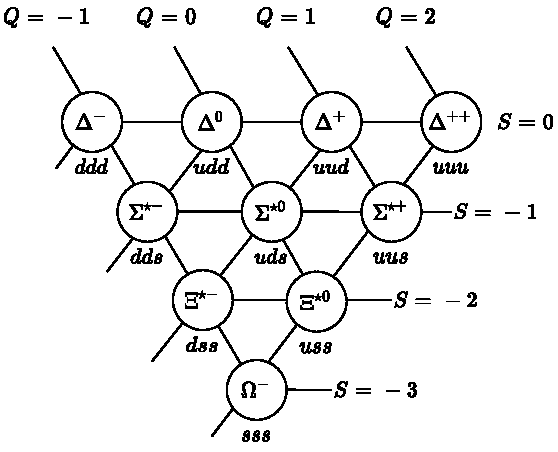
\includegraphics[width=0.7\linewidth]{baryon}
		\end{center}
		
		\item \begin{minipage}[t]{0.6\textwidth}
			For the ball to experience gravity on Earth, \begin{align*}
				y & = \frac{g}{2} t^2 = \frac{g}{2c^2} \left(ct\right)^2
			\intertext{From the diagram,}
				ct & = R_c \sin \theta \\
				y & = R_c(1 - \cos \theta) \\
				\left( 1 - \cos \theta \right) R_c & = \frac{1}{2} \frac{g}{c^2} {R_c}^2 \sin[2](\theta) \\
				\frac{1-\cos\theta}{\sin[2](\theta)} & = \frac{1}{2} \frac{g}{c^2} {R_c} 
				\intertext{Since $\frac{1-\cos\theta}{\sin[2](\theta)} \approx \frac{1}{2}$ for $\theta \approx 0$, }
				R_c & \approx \frac{c^2}{g} \approx \SI{9.18e15}{\m}
			\end{align*}
		\end{minipage}
		\begin{minipage}[t]{0.4\textwidth}
			~ \\
			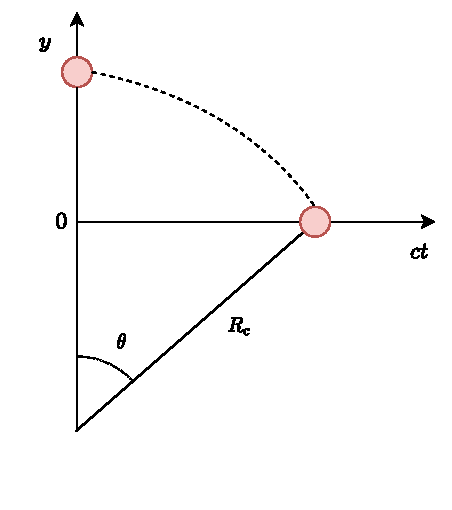
\includegraphics[width=\linewidth]{finalspacetime}
		\end{minipage}
		
	\end{enumerate}
\end{document}